%%%%%%%%%%%%%%%%%%%%%%%%%%%%%%%%%%%%%%%%%%%%%%%%%%%%%%%%%%%%%%%%%%%%%%%%%%%%%%%%
% Inicializálás                                                                %
%%%%%%%%%%%%%%%%%%%%%%%%%%%%%%%%%%%%%%%%%%%%%%%%%%%%%%%%%%%%%%%%%%%%%%%%%%%%%%%%

%%%%%%%%%%%%%%%%%%%%%%%%%%%%%%%%%%%%%%%%%%%%%%%%%%%%%%%%%%%%%%%%%%%%%%%%%%%%%%%%
% Papírméret, betűméret, margó, magyar karakterek                              %
%%%%%%%%%%%%%%%%%%%%%%%%%%%%%%%%%%%%%%%%%%%%%%%%%%%%%%%%%%%%%%%%%%%%%%%%%%%%%%%%

\documentclass[a4paper,12pt]{article}
\special{papersize=210mm,297mm}

\usepackage{anysize}
\marginsize{2.5cm}{2.5cm}{2.5cm}{2.5cm}

\usepackage[utf8]{inputenc}
\usepackage[magyar]{babel}

%%%%%%%%%%%%%%%%%%%%%%%%%%%%%%%%%%%%%%%%%%%%%%%%%%%%%%%%%%%%%%%%%%%%%%%%%%%%%%%%
% Fedlap inicializálása                                                        %
%%%%%%%%%%%%%%%%%%%%%%%%%%%%%%%%%%%%%%%%%%%%%%%%%%%%%%%%%%%%%%%%%%%%%%%%%%%%%%%%

\usepackage{fedlap}

\csapat{unexpected\_exceptions}{59}
\konzulens{Ferencz Endre}

\taga{Biró Loránd}{NCZAGL}{lol.kylerrr@gmail.com}
\tagb{Kanyó Tibor}{NXWUKE}{kanyo.tibi@gmail.com}
\tagc{Magyar Dániel}{SUFFGT}{samuraidanm@gmail.com}
\tagd{Tarjáni Tamás}{S499KV}{tarjanitomi@gmail.com}
\tage{Vajsz Kornél}{VUYNAW}{roncsipar@gmail.com}

%%%%%%%%%%%%%%%%%%%%%%%%%%%%%%%%%%%%%%%%%%%%%%%%%%%%%%%%%%%%%%%%%%%%%%%%%%%%%%%%
% Fejléc és lábléc                                                             %
%%%%%%%%%%%%%%%%%%%%%%%%%%%%%%%%%%%%%%%%%%%%%%%%%%%%%%%%%%%%%%%%%%%%%%%%%%%%%%%%

\usepackage{fancyhdr}

\setlength{\headheight}{1.4em}
\setlength{\headsep}{2em}

\fancyhf{}
\fancyhead[OL] { \leftmark{} }
\fancyhead[OR] { \tmpcsapat }
\fancyfoot[OC] { \thepage }
\fancyfoot[OR] { \tmpdatum }

\pagestyle{fancy}

%%%%%%%%%%%%%%%%%%%%%%%%%%%%%%%%%%%%%%%%%%%%%%%%%%%%%%%%%%%%%%%%%%%%%%%%%%%%%%%%
% Napló                                                                        %
%%%%%%%%%%%%%%%%%%%%%%%%%%%%%%%%%%%%%%%%%%%%%%%%%%%%%%%%%%%%%%%%%%%%%%%%%%%%%%%%

\usepackage{longtable}

\newenvironment{journal}
{
	\hbadness 10000
	\begin{longtable}{|p{60pt}|l|l|p{216pt}|}
	\hline
	\textbf{Kezdet} & \textbf{Időtartam} & \textbf{Résztvevők} & \textbf{Leírás} \\
	\hline
	\endfirsthead
	\hline
	\textbf{Kezdet} & \textbf{Időtartam} & \textbf{Résztvevők} & \textbf{Leírás} \\
	\hline
	\endhead
}
{
	\end{longtable}
}

\newcommand{\journalentry}[4]
{
	{#1} & {#2} óra & \parbox{50pt}{#3} & {#4} \\
	\hline
}

%%%%%%%%%%%%%%%%%%%%%%%%%%%%%%%%%%%%%%%%%%%%%%%%%%%%%%%%%%%%%%%%%%%%%%%%%%%%%%%%
% UseCase leírás                                                               %
%%%%%%%%%%%%%%%%%%%%%%%%%%%%%%%%%%%%%%%%%%%%%%%%%%%%%%%%%%%%%%%%%%%%%%%%%%%%%%%%

\newenvironment{usecase}
{
	\hbadness 10000
	\begin{longtable}[l]{|p{100pt}|p{328pt}|}
	\hline
	\endfirsthead
	\hline
	\endhead
}
{
	\hline
	\end{longtable}
}

\newcommand{\usecaseentry}[2]
{
	\hline
	\textbf{#1} & {#2}\\
}

%%%%%%%%%%%%%%%%%%%%%%%%%%%%%%%%%%%%%%%%%%%%%%%%%%%%%%%%%%%%%%%%%%%%%%%%%%%%%%%%
% FileList leírás                                                               %
%%%%%%%%%%%%%%%%%%%%%%%%%%%%%%%%%%%%%%%%%%%%%%%%%%%%%%%%%%%%%%%%%%%%%%%%%%%%%%%%

\newenvironment{filelist}
{
	\hbadness 10000

	\begin{longtable}{|p{145pt}|p{35pt}|p{63pt}|p{163pt}|}
	\hline
	\textbf{Fájl neve} & \textbf{Méret} & \textbf{Keletkezés ideje} & \textbf{Tartalom} \\
	\hline
	\endfirsthead
	\hline
	\textbf{Fájl neve} & \textbf{Méret} & \textbf{Keletkezés ideje} & \textbf{Tartalom} \\
	\hline
	\endhead
}
{
	\end{longtable}
}

\newcommand{\filelistentry}[4]
{
	{#1} & {#2} b & {#3} & {#4} \\
	\hline
}
%%%%%%%%%%%%%%%%%%%%%%%%%%%%%%%%%%%%%%%%%%%%%%%%%%%%%%%%%%%%%%%%%%%%%%%%%%%%%%%%
% Egyebek                                                                      %
%%%%%%%%%%%%%%%%%%%%%%%%%%%%%%%%%%%%%%%%%%%%%%%%%%%%%%%%%%%%%%%%%%%%%%%%%%%%%%%%

\usepackage{graphicx}		% Kepek beillesztesehez
\usepackage{epstopdf}		% EPS fajlok felismeresehez
\graphicspath{{Images/}}	% Az Images mappaban keresse a kepeket

\anyag{4. Analízis modell kidolgozása II.}
\datum{2012. március 4.}
\setcounter{section}{3}

%%%%%%%%%%%%%%%%%%%%%%%%%%%%%%%%%%%%%%%%%%%%%%%%%%%%%%%%%%%%%%%%%%%%%%%%%%%%%%%%
% Dokumentum                                                                   %
%%%%%%%%%%%%%%%%%%%%%%%%%%%%%%%%%%%%%%%%%%%%%%%%%%%%%%%%%%%%%%%%%%%%%%%%%%%%%%%%

\begin{document}

\fedlap

\section{Analízis modell kidolgozása}

\subsection{Objektum katalógus}

\subsubsection{GameLogic package}

\textbf{Vector2}: Egyszerű két dimenziós vektort megvalósító osztály.

\textbf{IBounds}: A pályaelemen található blokkok formáját fogja össze. Rendelkezik valós pozícióval és mérettel, valamint képes eldönteni, hogy egy másik ily osztállyal érintkezik-e és hogy egy adott pont benne van-e.

\textbf{TriangleBounds}: Háromszög alakzatot reprezentáló osztály, mely az ütközések kiszámításakor a háromszögnél használatos számításokkal dolgozik.

\textbf{RectangleBounds}: Egy téglalap alakzatot reprezentáló osztály. Ütközésdetektálás során téglalapként működik.

\textbf{GameObject}: Ezek a játékban szereplő objektumok. Tartalmazza, hogy melyik pályaelemben található az adott objektum, illetve hogy azon belül hol található, ezt az őt magába foglaló alakzatok pozíciója segítségével tárolja. Továbbá képes meghatározni, hogy érintkezik-e másik játékban szereplő objektummal.

\textbf{LevelPart}: Egy pályaelemet reprezentáló osztály. Tárolja az adott pályaelemhez tartozó blokkokat, valamint azt, hogy melyik pályaelemekkel szomszédos és hogy hova lehet átmenni róla.

\textbf{Level}: Ez a fő vezérlő osztály az egész játéklogikában. Tárolja azokat pályaelemet, amikből az adott pálya áll, továbbá ő intézi a pályaelemek tili-toli csúsztatását és a játék állapotának figyelését (teljesítettük-e már).

\textbf{Block}: Egy faldarabot jelképező játék objektum. 

\textbf{KeyHolder}: Egy kulcs helyét jelző játék objektum, azt tárolja van-e ott még kulcs.

\textbf{Door}: Egy üres GameObject osztály, mely csak azt reprezentálja, hogy helyileg hova kell menni a pálcikaemberrel, amennyiben megszereztük az összes kulcsot a pályán.

\textbf{Player}: A játékost reprezentáló játékobjektum, a játékos mozgását vezérli az inputok alapján.

\textbf{Direction}: Egy felsorolás amivel irányt jelezhetünk, többek között a pályaelemek csúsztatásának irányát adhatjuk meg vele.

\subsection{Osztályok leírása}

Az osztályok leírása során, amely osztálynál nem szerepel egy-egy tulajdonság, például \textbf{Ősosztály} vagy \textbf{Interfész}, az értelemszerűen azt jelöli, hogy az adott osztály nem rendelkezik vele. Az első három osztályt tartalmazó package az analízis modellhez szorosan nem tartozik hozzá, ezért a leírásuk csak a szekvenciadiagramok értelmezését segíti.

\subsubsection{LevelDescriptor}
	\begin{description}
		\item[Felelősség] \hfill \\
		Egy pálya felépítéséhez szükséges leíró információkat tárolja. A mérete legalább 1x2 vagy 2x1 kell hogy legyen.
		
		\item[Attribútumok]\hfill \\
		\textbf{\emph{int Width}}: pályaelemek száma egy sorban
		
		\textbf{\emph{int Height}}: pályaelemek száma egy oszlopban
		
		\textbf{\emph{LevelPartDescriptor[] Parts}}: az adott pályához tartozó pályaelemek listája
		
		\textbf{\emph{LevelObjectDescriptor}}: a pályán szereplő minden objektumot tartalmazó lista
				
		\item[Metódusok]\hfill \\
		\textbf{\emph{LevelDescriptor load(string)}}: betölti a megadott fájlból a pálya leíró objektumot.
						
	\end{description}

\subsubsection{LevelObjectDescriptor}
	\begin{description}
		\item[Felelősség] \hfill \\
		A pályán szereplő objektumok leírója.
		
		\item[Attribútumok]\hfill \\
		\textbf{\emph{int X}}: az adott objektum a pályaelemen való hollétének x koordinátája
		
		\textbf{\emph{int Y}}: az adott objektum pályaelemen való hollétének y koordinátája
		
		\textbf{\emph{int LevelPartIndex}}: a tartalmazó pályaelem indexe
		
		\textbf{\emph{LevelObjectType Type}}: az objektum típusa
						
	\end{description}

\subsubsection{LevelObjectType}
	\begin{description}
		\item[Felelősség] \hfill \\
		A pályán elhelyezhető objektumok típusainak felsorolása. A lehetséges értékek: Key, Door, Spawn.
		
	\end{description}

\subsubsection{RectangleBounds}
	\begin{description}
		\item[Felelősség] \hfill \\
		Egy téglalap alakzatot reprezentáló osztály. Ütközésdetektálásnál téglalapként való alakzatként adja vissza az irányvektort. A téglalap alakú blokkok, objektumok érintkezését tudjuk kezelni ezen osztállyal.
				
		\item[Interfészek] \hfill \\
		IBounds
		
	\end{description}

\subsubsection{TriangleBounds}
	\begin{description}
		\item[Felelősség] \hfill \\
		Háromszög alakzatot reprezentáló osztály. Ütközésdetektálásnál háromszögként való alakzatként adja vissza az irányvektort. Ezekkel tudjuk kezelni a ferde alakzatokat a pályaelemeken.
				
		\item[Interfészek] \hfill \\
		IBounds
		
	\end{description}

	
\subsubsection{IBounds}
	\begin{description}
		\item[Felelősség] \hfill \\
		 Minden GameObject helyét és méretét ez alapján határozzuk meg. Az ebből leszármaztatott osztály tudja, hogy metszi-e egy másik ugyan ilyen típusú objektum, és hogy egy adott pont benne van-e. Egyfajta hitboxként is funkcionál. 
		 
		\item[Attribútumok]\hfill \\
		\textbf{\emph{float X}}: az alakzat x koordinátája
		
		\textbf{\emph{float Y}}: az alakzat y koordinátája
		
		\textbf{\emph{float Width}}: a befoglaló téglalap szélessége
		
		\textbf{\emph{float Height}}: a befoglaló téglalap magassága
		
		\item[Metódusok]\hfill \\		
		\textbf{\emph{Vector2 GetIntersectionDepthWidth(IBounds)}}: visszaadja egy vektorban, hogy a paraméterül adott objektumba mily mértékben vagyunk benne ütközés esetén.
		
		\textbf{\emph{bool Intersects(IBounds)}}: eldönti, hogy a paraméterül kapott másik ilyen objektummal metszik-e egymást
		
		\textbf{\emph{bool Contains(float x, float y)}}: egy (x,y) koordinátájú pontról megmondja, hogy az objektum területén van-e
								
	\end{description}

\subsubsection{GameObject}
	\begin{description}
		\item[Felelősség] \hfill \\
		Minden, a pályaelemekben található objektum (Block, KeyHolder, Door, Player) ebből az absztrakt osztályból származik. Egy Rectangle osztály segítségével tárolja a méretét és helyét, illetve tudja, hogy melyik pályaelemben található. A tárolt Rectangle objektum Intersects metódusára építve végzi az ütközésdetekciót. A GameObject meguk frissítik a pozíciójukat.
		
		\item[Attribútumok]\hfill \\
		\textbf{\emph{LevelPart LevelPart}}: referencia arra a pályaelemre, amelyikben van
		
		\textbf{\emph{Rectangle Location}}: egy Rectangle objektum, a pozíció és méret tárolásához
		
		\item[Metódusok]\hfill \\
		\textbf{\emph{bool CollidesWith(GameObject other)}}: ütközésdetektáló metódus. A Rectangle Intersects függvényétől annyiban különbözik, hogy azt is vizsgálja, hogy a két vizsgált objektum egy pályaelemben található-e (vagyis ténylegesen metszik-e egymást).
						
	\end{description}

\subsubsection{Vector2}
	\begin{description}
	\item[Felelősség] \hfill \\
	Egy kétdimenziós vektorként működik.
	\item[Attribútumok] \hfill \\
	\textbf{\emph{float X}}: a vektor x koordinátájának nagysága
	
	\textbf{\emph{float Y}}: a vektor y koordinátájának nagysága
	\end{description}

\subsubsection{LevelPart}
	\begin{description}
		\item[Felelősség] \hfill \\
		Egy pályaelemet reprezentáló osztály. Tárolja a helyét a pályán belül, a benne előforduló blokkokat, a szomszédos pályaelemeket, illetve, hogy ezek közül melyikbe lehet átmenni.

		\item[Attribútumok]\hfill \\		
		\textbf{\emph{int X}}: a pályaelem X irányú pozíciója
		
		\textbf{\emph{int Y}}: a pályaelem Y irányú pozíciója
		
		\textbf{\emph{Block[] Blocks}}: a pályaelemben szereplő blokkok
		
		\textbf{\emph{LevelPart[] Neighbours}}: a szomszédos pályaelemeket tároló Direction szerint címezhető tábla.
		
		\textbf{\emph{bool[] Passabilities}}: a különböző irányokba való átjárhatóságot tároló Direction szerint címezhető tábla.
		
		\item[Metódusok]\hfill \\
		\textbf{\emph{void Update()}}: újraszámolja a Neighbours és a Passabilities listákat
	
		\textbf{\emph{LevelPart GetNeighbour()}}: visszaadja azt az üres résszel szomszédos pályaelemet, amelyiket mozgatni kell a távoli nézetben

		\textbf{\emph{bool[] GetSide(Direction)}}: visszaadja a megadott oldalon található blokkokat (pl. a GetSide(Down) függvényhívás visszatérési értéke az adott LevelPart alján lévő blokkok tömbje - true, ha van blokk, false, ha nincs)
		
		\textbf{\emph{bool IsPassableTo(Direction)}}: megadja, hogy a játékos elhagyhatja-e a pályaelemet az adott irányba
	\end{description}
	
\subsubsection{Level}
	\begin{description}
		\item[Felelősség] \hfill \\
		Ez a fő vezérlő osztály az egész játéklogikában. Ő hozza létre a játékos, az ajtó, a kulcs helyek, a pályát alkotó pályaelemeket vezérlő osztályokat. Ez az osztály végzi a játék állapotának frissítését és a pályaelemek tili-toli módú irányítását is.
		
		\item[Attribútumok]\hfill \\
		\textbf{\emph{int Width}}: a pálya szélessége
		
		\textbf{\emph{int Height}}: a pálya magassága
		
		\textbf{\emph{LevelPart[] Parts}}: a pályát alkotó pályaelemek listája
		
		\textbf{\emph{KeyHolder[] KeyHolders}}: mindezon helyek a pályán, ahol van/volt kulcs
		
		\textbf{\emph{Door Door}}: a pálya végét jelképező ajtó
		
		\textbf{\emph{bool isCompleted}}: ez az attribútum jelzi a pálya állapotát.
		
		\textbf{\emph{Player Player}}: a játékost leíró Player objektum
		
		\item[Metódusok]\hfill \\
		\textbf{\emph{void Update()}}: megvizsgálja a Player aktuális pozícióját és frissíti a pálya és a KeyHolder-ek állapotait ha szükséges.
		
		\textbf{\emph{void Slide(Direction direction)}}: egy pályaelem csúsztatását valósítja meg. Pl. egy felfele irányú csúsztatás esetén az üres terület alatti pályaelemet mozgatja felfele (amennyiben van alatta pályaelem), majd frissíti a LevelPart-okat hogy az aktuális átjárhatóságokat tárolja.
						
	\end{description}
	
\subsubsection{Block}
	\begin{description}
		\item[Felelősség] \hfill \\
		Nem átjárható, a falat reprezentáló GameObject, aktív szerepe nincs.
		
		\item[Ősosztályok]\hfill \\
		GameObject absztrakt osztályból származik
						
	\end{description}
	
\subsubsection{KeyHolder}
	\begin{description}
		\item[Felelősség] \hfill \\
		Egy kulcs lehetséges helyét jelölő GameObject. Tárolja, hogy ott van-e még a kulcs, vagy a játékos már felvette.
		
		\item[Ősosztályok]\hfill \\
		GameObject absztrakt osztályból származik
		
		\item[Attribútumok]\hfill \\
		\textbf{\emph{bool HasKey}}: van-e még nála kulcs, vagy a játékos már felvette
						
	\end{description}
	
\subsubsection{Door}
	\begin{description}
		\item[Felelősség] \hfill \\
		A pálya végét jelentő GameObject, csak az ajtó pozícióját tárolja.
		
		\item[Ősosztályok]\hfill \\
		GameObject absztrakt osztályból származik
						
	\end{description}
	
\subsubsection{Player}
	\begin{description}
		\item[Felelősség] \hfill \\
		A játékos által irányítható avatár, a kapott inputok alapján a saját mozgatásáért felelős.
		
		\item[Ősosztályok]\hfill \\
		GameObject absztrakt osztályból származik
		
		\item[Metódusok]\hfill \\
		\textbf{\emph{void Update(float time, bool goLeft, bool goRight, bool jump)}}: frissíti a Player helyzetét attól függően, hogy éppen milyen inputokat kap.
		
		\textbf{\emph{void ApplyPhysics()}}: a Player mozgását a valós fizikai világot megközelítően igazítja.
				
		\textbf{\emph{void HandleCollisions()}}: korrigálja a Player pozícióját, amennyiben az egy ütközés során indokolttá válik. Például az ütközésvizsgálat szerint pont benne van már a falban, akkor odébbteszi annyival a játékost, hogy pont még ne érjen bele.
						
	\end{description}
	
\subsubsection{Direction}
	\begin{description}
		\item[Felelősség] \hfill \\
		Egy felsorolás amivel irányt jelezhetünk, többek között a tili-toli csúsztatás irányát adhatjuk meg vele. Lehetséges értékei: Left, Up, Right, Down.
	\end{description}
	
\subsection{Statikus struktúra diagramok}
\begin{center}
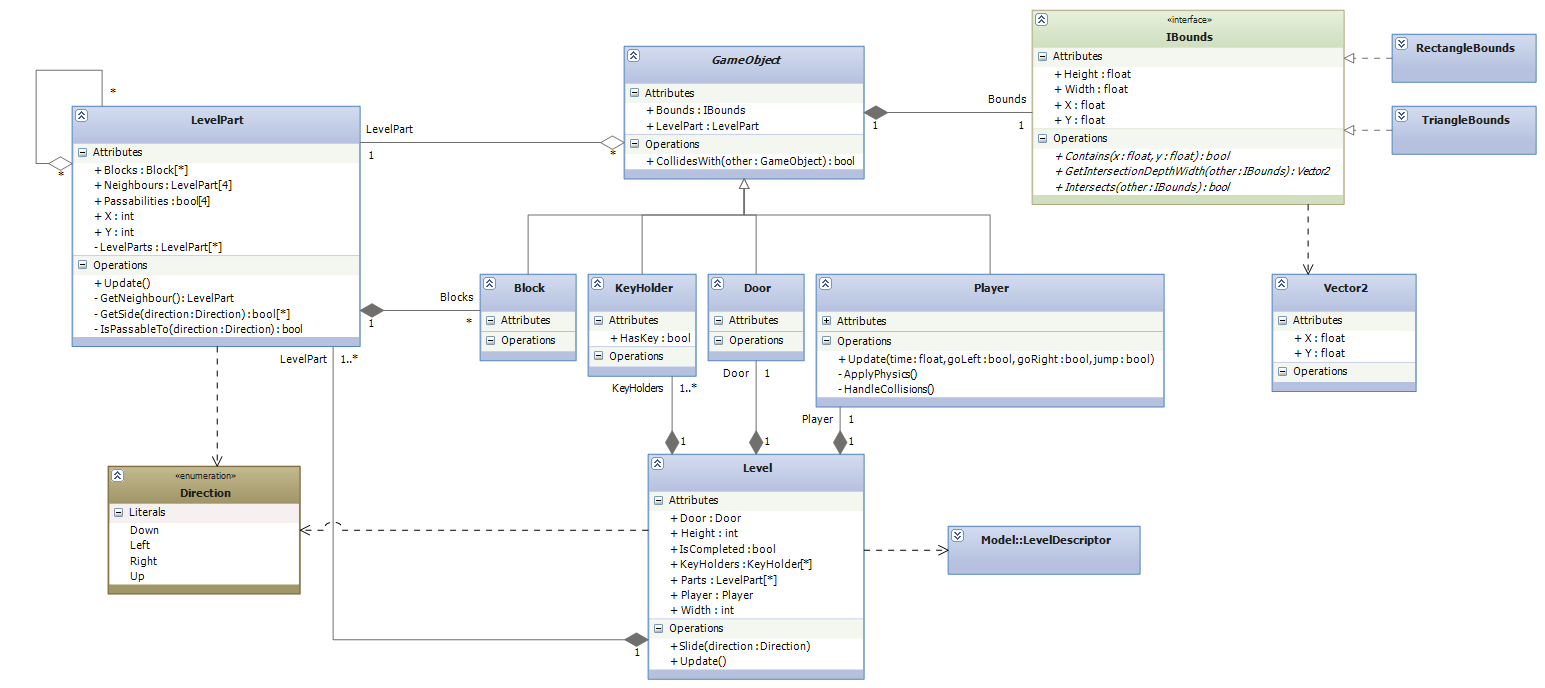
\includegraphics[scale=0.55,angle=90]{04_SSD_GameLogic.png}
\newpage
\end{center}

\subsection{Szekvencia diagramok}

\subsubsection{Játék inicializálása}
\begin{center}
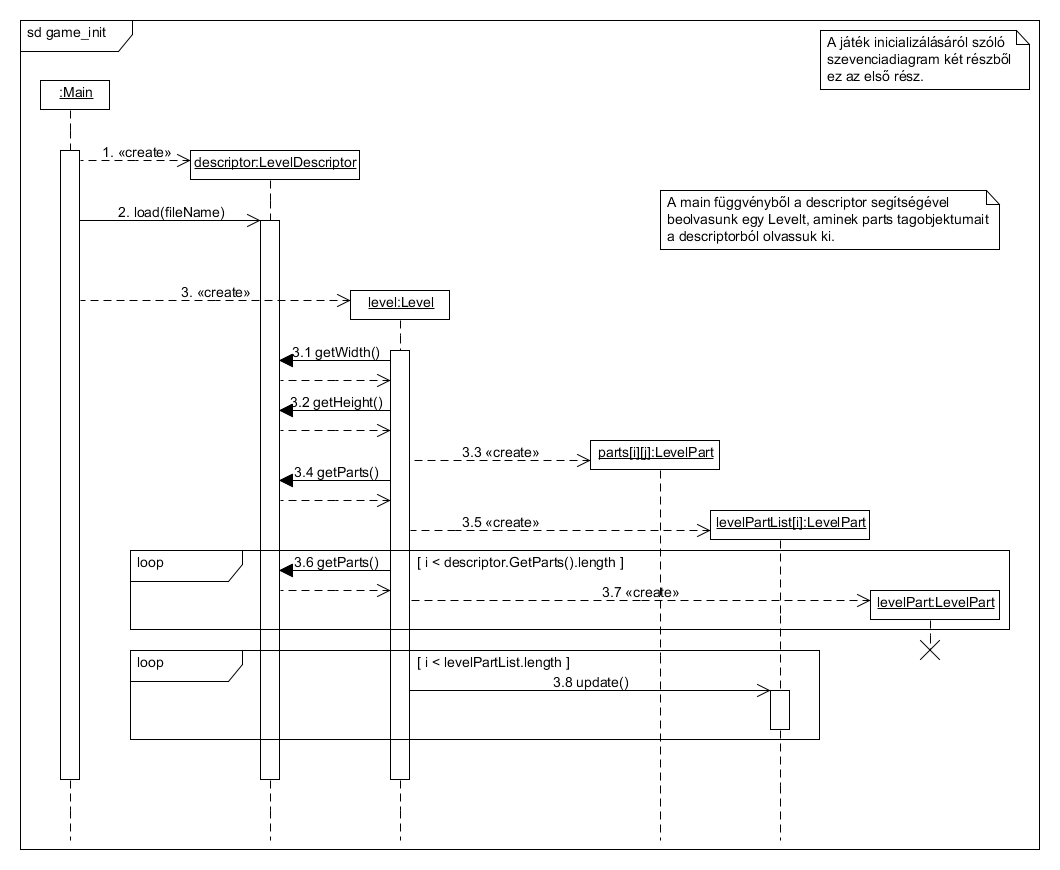
\includegraphics[scale=0.51,angle=90]{03_sdGameInita.png}
\newpage
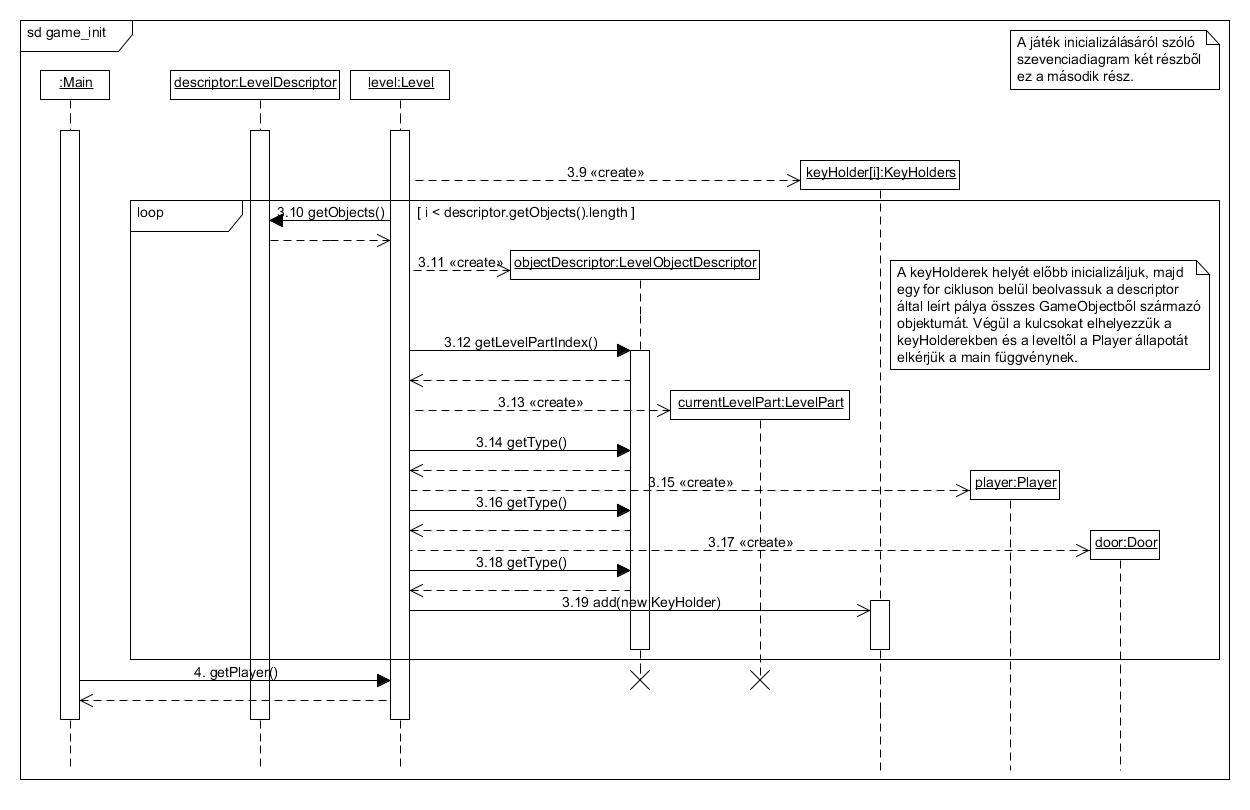
\includegraphics[scale=0.50,angle=90]{03_sdGameInitb.png}
\newpage
\end{center}

\subsubsection{Illeszkedésvizsgálat}
\begin{center}
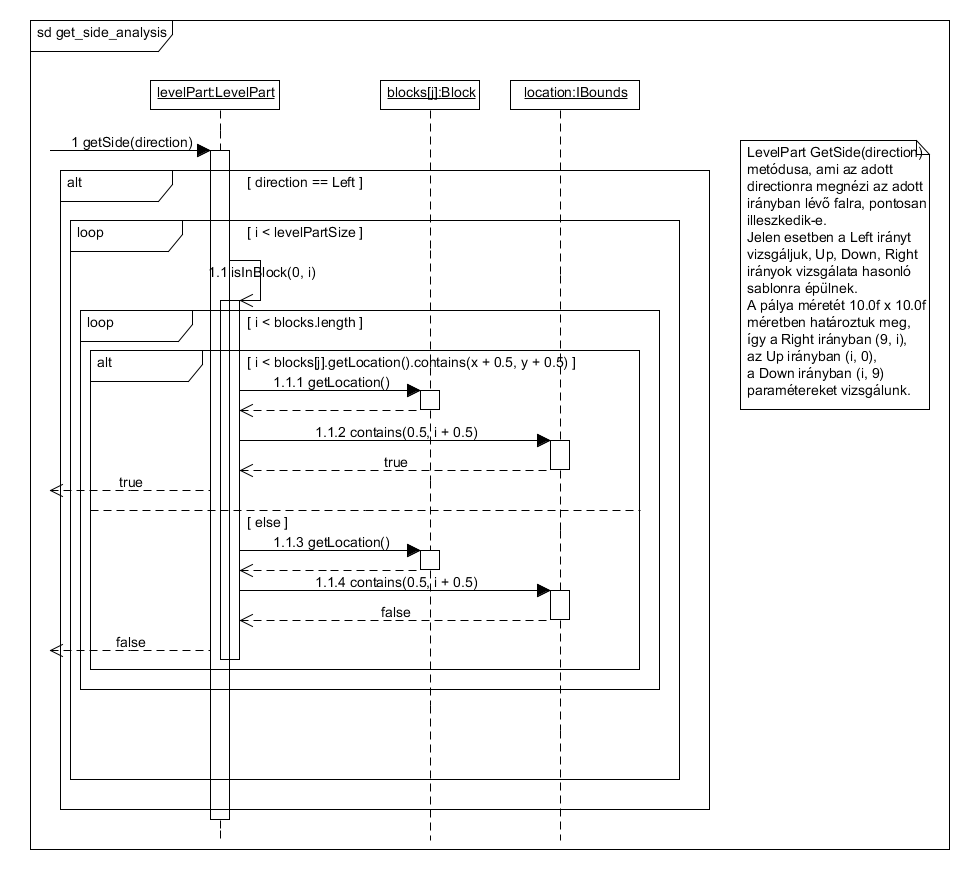
\includegraphics[scale=0.46]{03_sdGetSideAnalysis.png}
\newpage
\end{center}

\subsubsection{Csúsztatásvizsgálat}
\begin{center}
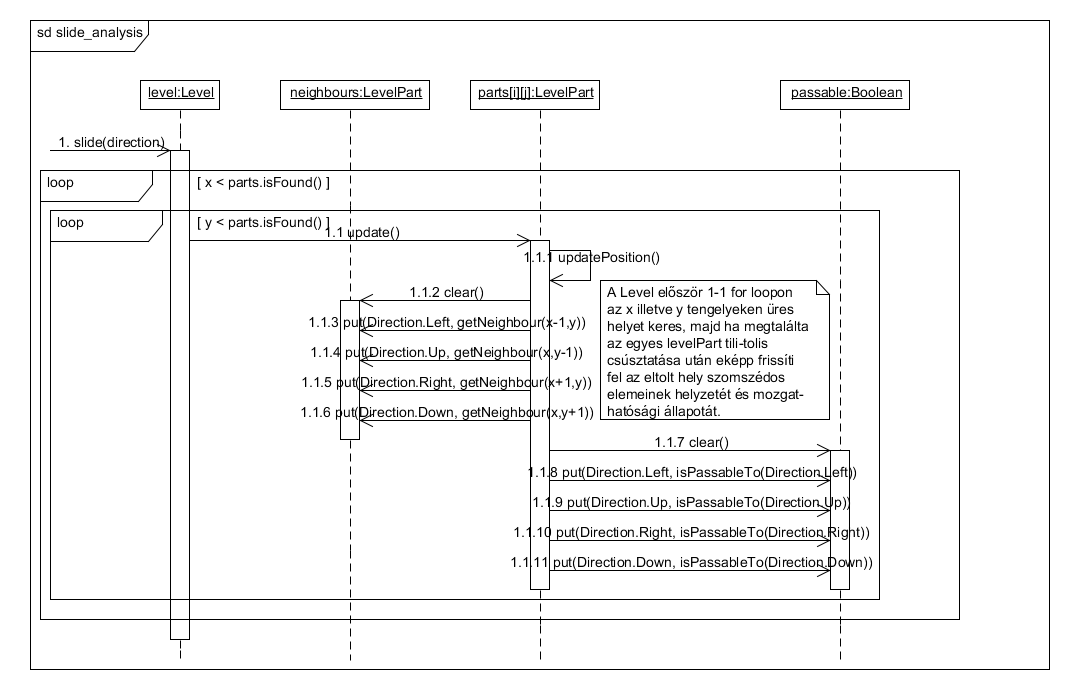
\includegraphics[scale=0.60,angle=90]{03_sdSlideAnalysis.png}
\newpage
\end{center}

\subsubsection{Ütközésvizsgálat}
\begin{center}
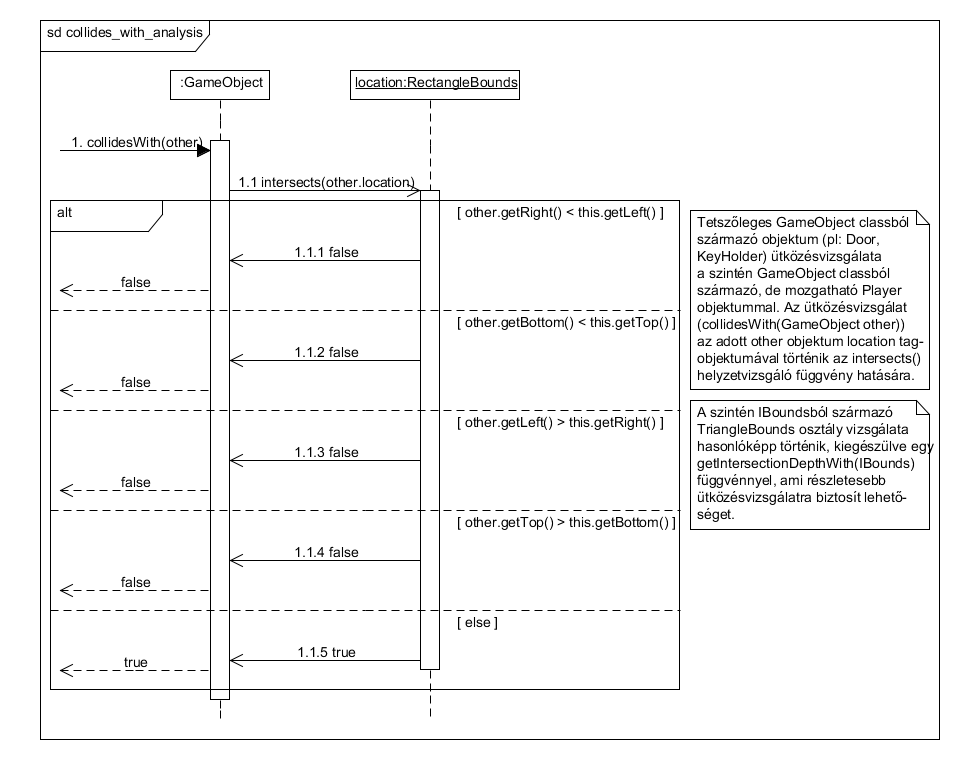
\includegraphics[scale=0.47]{03_sdCollidesWithAnalysis.png}
\end{center}

\subsubsection{Főciklus}
\begin{center}
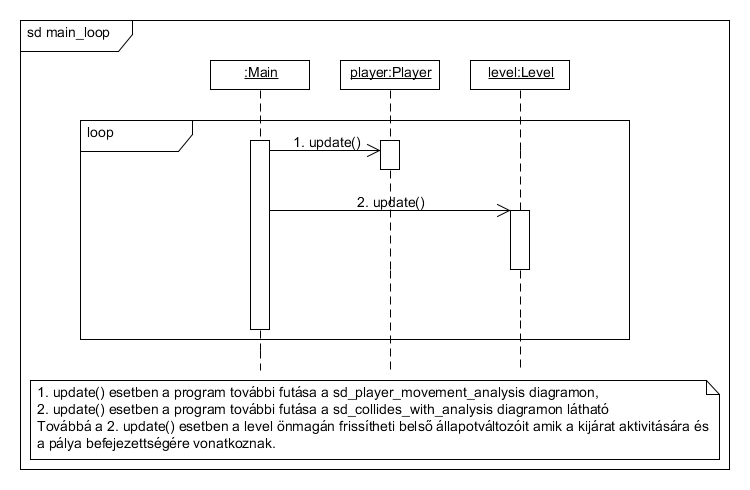
\includegraphics[scale=0.50]{03_sdMainLoop.png}
\newpage
\end{center}

\subsubsection{Játékos mozgása}
\begin{center}
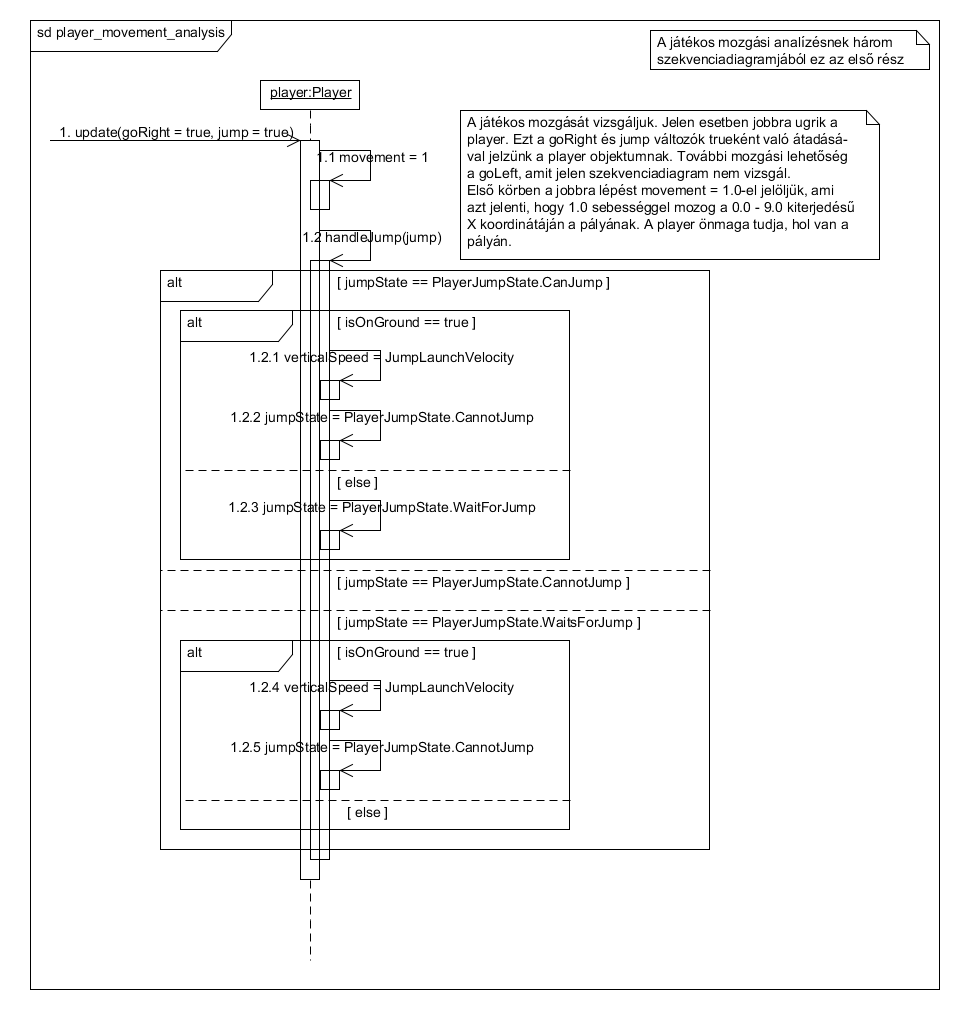
\includegraphics[scale=0.40]{03_sdPlayerMovementAnalysisa.png}
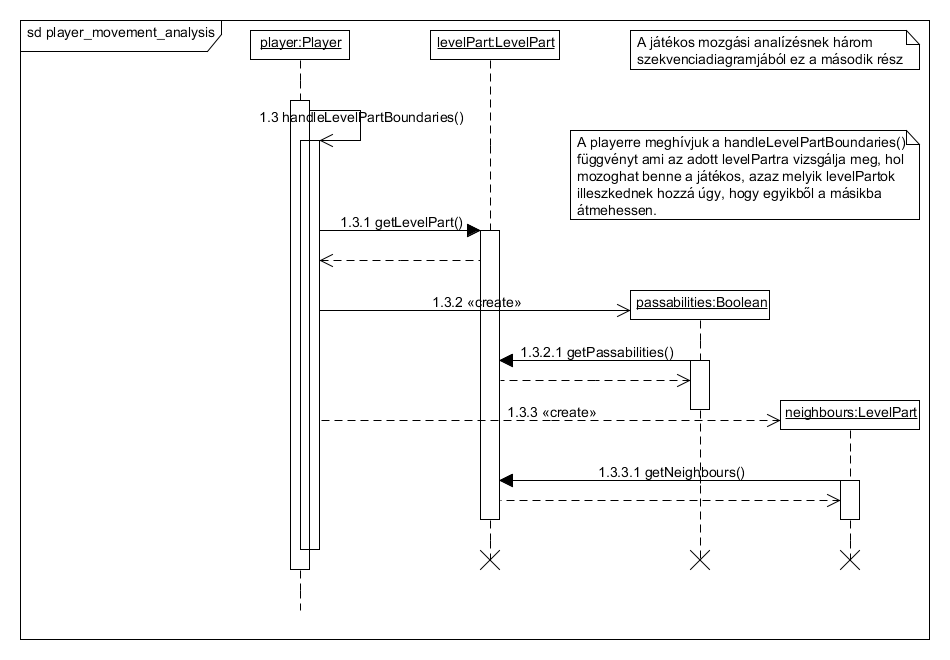
\includegraphics[scale=0.40]{03_sdPlayerMovementAnalysisb.png}
\newpage
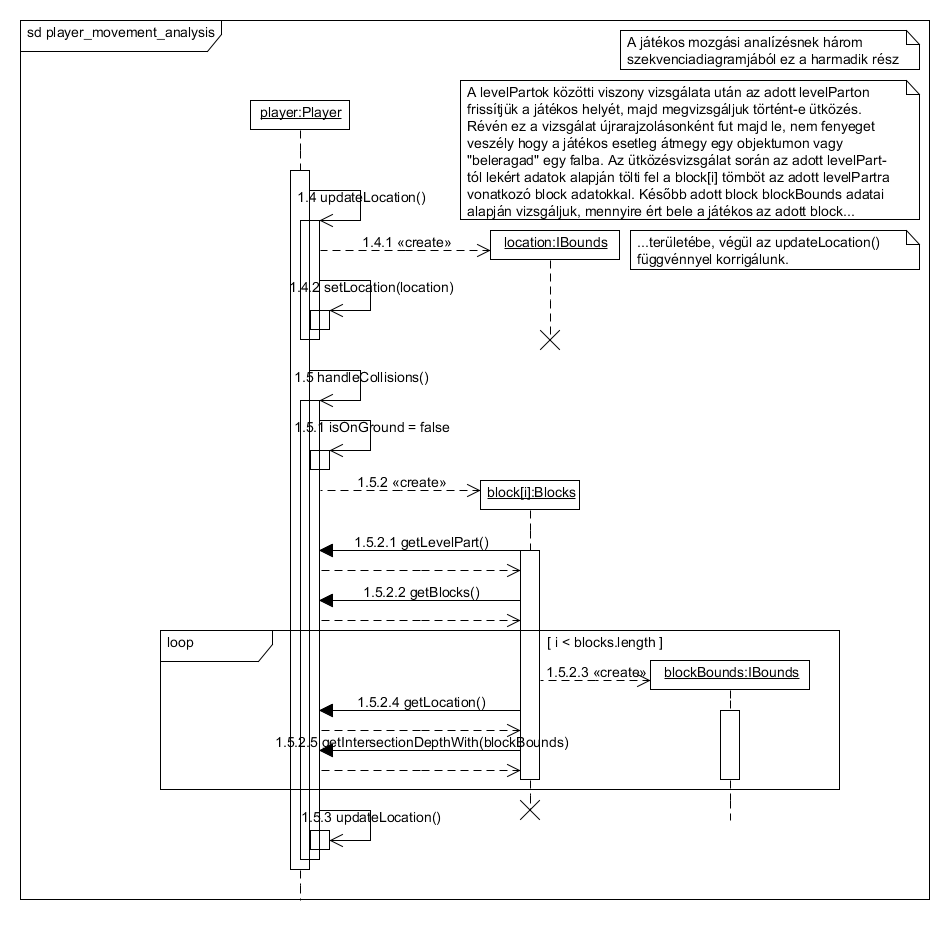
\includegraphics[scale=0.45]{03_sdPlayerMovementAnalysisc.png}
\newpage
\end{center}

\subsection{State-chartok}


\subsubsection{Level és KeyHolder osztály viselkedése}
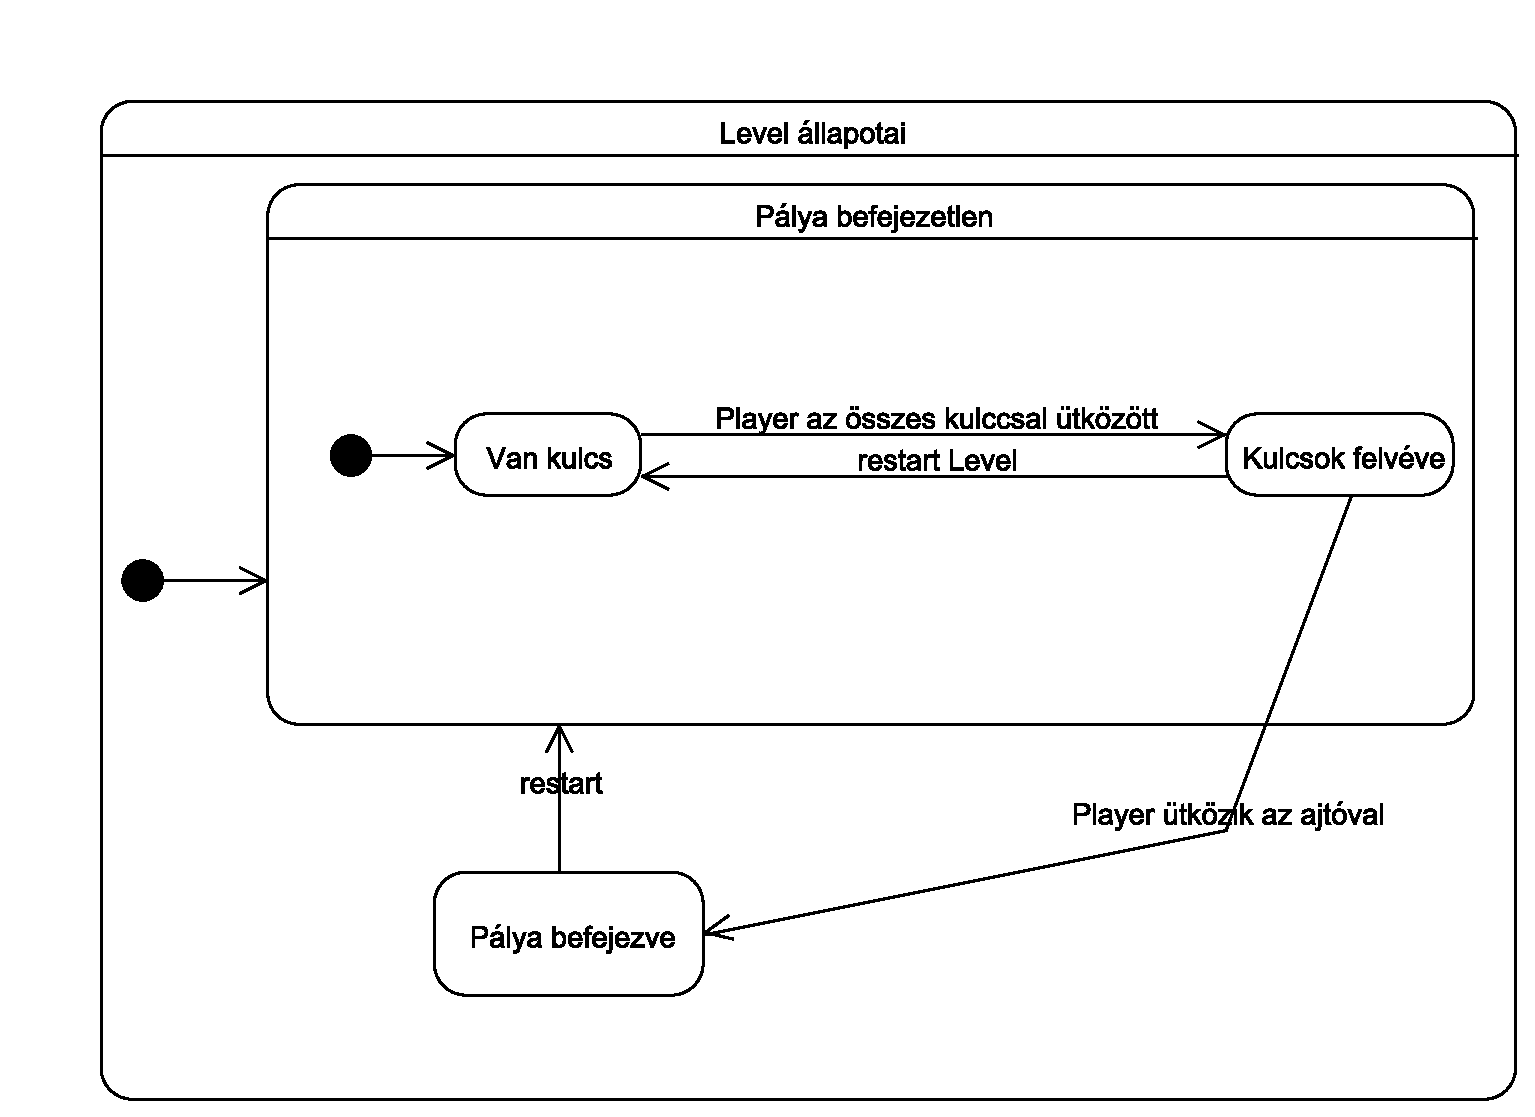
\includegraphics[scale=0.65]{03_statechart_Level2.eps}
\newpage
\subsection{Napló}

\begin{journal}

\journalentry{2012.02.28. 12:30}{1}{Bíró, Kanyó, Tarjáni, Vajsz}{Személyes értekezlet. A konzultáció tapasztalatait megbeszéltük, pár apró változtatást eszközöltünk a projekten.}

\journalentry{2012.03.03. 21:15}{3,75}{Vajsz}{A szekvenciadiagramokat visszaállítottam majd a konzultáción elhangzottak alapján frissítettem, újratördeltem és kommentekkel láttam el. A kapott szekvenciadiagramokat kiexportáltam és beleraktam egy új \LaTeX{} projektbe.}

\journalentry{2012.03.04. 9:15}{1}{Kanyó}{A Model package-et és a hozzá tartozó osztályok leírását eltávolítottam. Az újabb metódusok formális leírását megcsináltam.}
\journalentry{2012.03.04. 9:45}{1}{Tarjáni}{Osztály- és metódusleírások szerkesztése.}
\journalentry{2012.03.04. 12:00}{0,7}{Kanyó}{Az IBounds interfésszel bővített UML alapján létrejött újabb osztályok formális leírása.}
\journalentry{2012.03.04. 23:45}{0,5}{Vajsz}{A levlistán elhangzottak alapján pár kisebb javítás eszközölése a szekvenciadiagramokon.}


\end{journal}

\end{document}